% !TEX root = ../thesis-sample.tex

\chapter{Now we know what they mean by ``advanced'' tactical training.} \label{chap:intro}

Here's an acronym \ac{CRTBP} and a symbol \ac{F}, followed by some random text.
Now what are the possibilities of warp drive? Cmdr Riker's nervous system has been invaded by an unknown microorganism. The organisms fuse to the nerve, intertwining at the molecular level. That's why the transporter's biofilters couldn't extract it. The vertex waves show a K-complex corresponding to an REM state. The engineering section's critical. Destruction is imminent. Their robes contain ultritium, highly explosive, virtually undetectable by your transporter.

Deflector power at maximum. Energy discharge in six seconds. Warp reactor core primary coolant failure. Fluctuate phaser resonance frequencies. Resistance is futile. Recommend we adjust shield harmonics to the upper EM band when proceeding. These appear to be some kind of power-wave-guide conduits which allow them to work collectively as they perform ship functions. Increase deflector modulation to upper frequency band.

\section{Float environments}
Theere are many possible float enviornments, and this section will serve as an introduction and demonstration of each of them.
In addition, it offers the ability to ensure that this template actually follows the guidelines.

\subsection{Figures}\label{ssec:figures}

Here is a figure as shown in~\cref{fig:plain}.

\begin{figure}
    \centering
    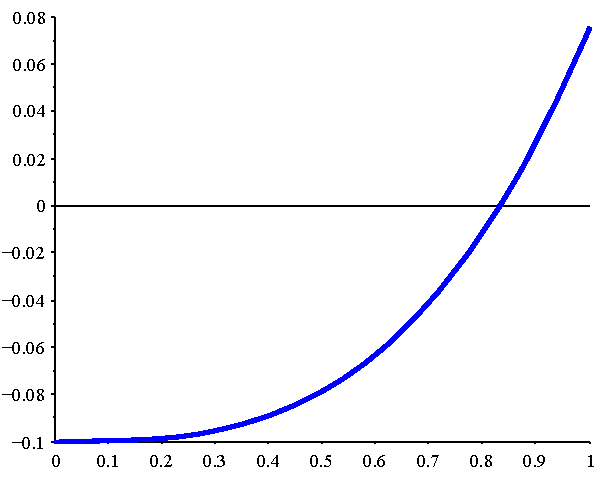
\includegraphics[width=0.5\textwidth]{figures/f1_plain.pdf}
    \caption[Short caption for TOC]{Long caption to appear in text\label{fig:plain}}
\end{figure}

\subsection{Tables}\label{ssec:tables}

here's a table in~\cref{tab:table}

\begin{table}
\begin{center}
    \begin{tabular}{ | l | l | l | p{5cm} |}
    \hline
    Day & Min Temp & Max Temp & Summary \\ \hline
    Monday & 11C & 22C & A clear day with lots of sunshine.  
    However, the strong breeze will bring down the temperatures. \\ \hline
    Tuesday & 9C & 19C & Cloudy with rain, across many northern regions. Clear spells 
    across most of Scotland and Northern Ireland, 
    but rain reaching the far northwest. \\ \hline
    Wednesday & 10C & 21C & Rain will still linger for the morning. 
    Conditions will improve by early afternoon and continue 
    throughout the evening. \\
    \hline
    \end{tabular}
    \caption[Short caption for table]{Long caption for text \label{tab:table}}
    \end{center}
\end{table}

\section{References and Citation}

\subsection{Clever referencing}
\LaTeX offers the powerful ability to automatically handle references using \verb+\label+ and a corresponding \verb+\ref+.
While~\cref{chap:intro} has more detail on some good practices for \LaTeX~that I've picked up.

\subsection{References}

Lots of famous people tend to write famous papers~\cite{newton1999}. 
Were they famous because or in-spite of their papers?
Regardless, they're famous now and we all should read them.
Certain people are so famous and do such great work that they invent a whole new field of study with a single paper~\cite{kalman1960,shannon1949}

\section{Math}

Here are some nice equations~\cref{prob_def,prob_def_constrained}

\begin{align}
\label{prob_def}
&\min_{s\subset W}\ J(s) = \sum_{i=1}^{l-1} H(s_j, s_{j+1}) \\
&\max_{s\subset W}\ P_{tr}(s) = \prod_{i=1}^{l-1} P_{tr}(s_j, s_{j+1}) \nonumber
\end{align}

\begin{align}
\label{prob_def_constrained}
&\min_{s\subset W}\ J(s) = \sum_{i=1}^{l-1} H(s_j, s_{j+1}) \\
&\text{subject to} \ P_{tr}(s)>\epsilon_{tr} \nonumber
\end{align}
